% ===========================================================================
% SECTION 5 — MPC FRAMEWORK
% Target: 800-1000 words
% ===========================================================================

\section{MPC Framework}
\label{sec:mpc_framework}

\subsection{nlmpc Formulation}
\label{subsec:nlmpc_formulation}

Closed-loop control is implemented with MATLAB's nonlinear MPC object
(\texttt{nlmpc}), instantiated separately for each surrogate with state
vector $x=[\omegar,\beta]$, output vector $y=x$ (identity output map),
manipulated variable $u=\betacmd$, and measured disturbance $V$. All
controllers share the sampling time $T_s = \SI{0.1}{s}$, prediction
horizon $N_p = 10$, and control horizon $N_c = 4$. The standard quadratic
cost (used by the Baseline, LLNFM, and PINN controllers) is

\begin{equation}
J = \sum_{k=1}^{N_p} \Big[ Q\,(\omegar(k)-\omegarated)^2
+ Q_2\,\beta(k)^2 + R\,(\Delta u(k))^2 \Big],
\label{eq:mpc_cost_standard}
\end{equation}

with tracking weight $Q=100$, a small pitch-regulation weight
$Q_2=0.01$ (encoded via \texttt{nlobj.Weights.OutputVariables}), and
control-rate weight $R=0.5$. Input constraints enforce the physical pitch
range $\beta \in [0\deg,25\deg]$ and the pitch rate limit
$|\Delta\beta| \le \dot\beta_{\max} T_s = \SI{0.8}{deg}$ per step
(from $\dot\beta_{\max}=\SI{8.0}{deg/s}$, Table~\ref{tab:turbine_params}).
The rotor-speed output constraint $\omegar \in [\omega_{\min}^{\text{bound}},
\omega_{\max}^{\text{bound}}]$ is controller-dependent, as detailed in
Section~\ref{subsec:surrogate_integration}. The SQP solver is configured
with bounded worst-case iteration cost
(\texttt{MaxIterations}$=30$, \texttt{MaxFunctionEvaluations}$=300$,
constraint/optimality/step tolerances of $10^{-4}$); this deviates from
nlmpc's default \texttt{MaxIterations}$=400$, which was found in early
testing to allow the SQP solver to run for over $20$ seconds per control
step when constraints were difficult to satisfy with an ML surrogate in
the loop (observed: $\SI{20624}{ms}$/step for LLNFM-MPC at simulation step
$k=480$). Because each SQP iteration evaluates the surrogate state
function multiple times for cost and constraint gradients, this cost
scales with surrogate inference latency — a recurring theme in the
feasibility analysis of Section~\ref{subsec:operational_feasibility}. A
real-time controller must have a bounded worst-case computation time
\citep{richter2012,xi2013}, so a
feasible-but-possibly-suboptimal solution within budget is preferred over
an unbounded search for the optimum.

\subsection{Surrogate Integration as State Function}
\label{subsec:surrogate_integration}

Each surrogate is wrapped as an nlmpc \texttt{StateFcn} with signature
$x^{+} = f(x,u,p_1,\ldots,p_n)$, where the parameter count
\texttt{NumberOfParameters} must match between the \texttt{StateFcn} and
any \texttt{CustomCostFcn} (confirmed empirically in R2024a: unused
trailing parameters are silently ignored rather than raising an error).
The controller signatures used are: Baseline
\texttt{sf\_baseline(x,u,V,p)} ($n=2$, the true physical plant
Eqs.~\eqref{eq:rotor_ode}--\eqref{eq:pitch_actuator}, no surrogate
involved); LLNFM and PINN \texttt{sf\_*(x,u,V,mdl)} ($n=2$); LSTM
\texttt{sf\_lstm(x,u,V,mdl,seq\_buf)} ($n=3$, carrying an explicit sequence
buffer); and GP \texttt{sf\_gp(x,u,V,mdl,omega\_ref,kappa)} ($n=4$, where
\texttt{omega\_ref} and \texttt{kappa} are unused by the state function
itself and passed only to satisfy the shared-parameter-count requirement
with \texttt{cost\_gp}, Section~\ref{subsec:gp_uncertainty_cost}).

The rotor-speed output constraint uses two distinct bounds for two
distinct failure modes. The Baseline controller, which evaluates the true
plant directly, uses a physics-based defense-in-depth floor
$\omegar \in [\SI{11.5}{rpm}, \omega_{\max}]$
($\omega_{\max}=\SI{13.31}{rpm}$); this bound is not load-bearing for
feasibility once the Region~II/III torque switching correction
(Section~\ref{subsec:torque_switching}) is in place, but is retained as a
cheap safeguard. The four surrogate controllers, in contrast, are
\emph{required} to be bounded within the Stage~1 training domain with a
$\SI{0.5}{rpm}$ safety margin, $\omegar \in [\SI{8.52}{rpm},
\SI{12.81}{rpm}]$: this constraint is not optional, since surrogate
predictions outside their training domain are unconstrained
extrapolations. This was discovered empirically — an early LLNFM-MPC run
without this bound drove $\omegar$ down to $\SI{7.55}{rpm}$ (outside the
then-current training range) while the pitch angle saturated at
$25\deg$, consistent with the surrogate losing sensitivity to the true
state once its input left the domain over which its rule base (or, more
generally, its learned response surface) was calibrated; a symptom-level
input-clamping fix at the surrogate's input boundary was found to mask
rather than resolve the underlying cause, and the correct fix is instead
to constrain the MPC's own admissible operating region.

\subsection{GP-MPC Uncertainty Cost (Gap-1)}
\label{subsec:gp_uncertainty_cost}

For the GP controller, the standard quadratic cost is replaced entirely
(\texttt{Optimization.ReplaceStandardCost = true}) with a custom cost
function that adds a predictive-uncertainty penalty over the prediction
horizon:

\begin{equation}
J_{\text{GP}} = \sum_{k=1}^{N_p} \Big[ Q\,(\omegar(k)-\omegarated)^2
+ Q_2\,\beta(k)^2 + R\,(\Delta u(k))^2
+ \kappa\,\sigma_{\omega}(k)^2 \Big],
\label{eq:gp_mpc_cost}
\end{equation}

where $\sigma_{\omega}(k)$ is the GP's predictive standard deviation on
the rotor-speed channel at the predicted state/input pair $k$ steps ahead
(re-queried from the GP model at every stage of the prediction horizon,
using the same input feature normalization as the state function), and
$\kappa=0.8$ is the uncertainty penalty weight. Because GP-v2's
hyperparameters are calibrated by marginal-likelihood optimization
(Section~\ref{subsubsec:gp_v2}) rather than left at default values, the
resulting $\sigma_\omega$ is a statistically meaningful (Bayesian)
uncertainty estimate rather than an arbitrary scale, which is the
methodological justification for using it directly as an MPC cost penalty:
the controller is driven to prefer trajectories that stay within regions
of the state space where the surrogate is confident, in addition to
tracking performance. We note as an implementation detail that the nlmpc
internal \texttt{data} struct in R2024a does not expose a
\texttt{data.Weights} field (verified by inspecting
\texttt{fieldnames(data)}, which lists \texttt{Ts},
\texttt{CurrentStates}, \texttt{LastMV}, \texttt{References},
\texttt{PredictionHorizon}, but no \texttt{Weights}); consequently $Q$,
$Q_2$, and $R$ are hardcoded inside \texttt{cost\_gp.m} to match
\texttt{stage0\_config.m}, with no automatic propagation if the
configuration changes — a documented limitation of the custom-cost
approach in this MATLAB version.

\subsection{Operational Feasibility Analysis}
\label{subsec:operational_feasibility}

This section reports a five-stage diagnostic investigation into why
several ML surrogates fail catastrophically inside the closed-loop SQP
solve despite being fast in isolation, and how this failure was
ultimately resolved. We report the investigation in the order it was
conducted, including negative results, because the sequence of ruled-out
hypotheses is itself informative for practitioners facing a similar
symptom.

\paragraph{Stage 1 --- Isolated inference latency is not predictive of
closed-loop cost.} An isolated benchmark calling each surrogate's state
function directly (bypassing \texttt{nlmpc} entirely, with randomized
inputs drawn from the training domain at every call, replicating how
SQP probes different state/input pairs) found per-call latencies in the
sub-millisecond to low-millisecond range for TCN, SW-MLP, and PINN-v2,
with only rare spikes (0--4 calls out of 250 exceeding \SI{50}{ms}) even
for LSTM. Table~\ref{tab:isolated_benchmark} reports the isolated
results.

\begin{table}[H]
\centering
\caption{Isolated state-function call latency (250 calls, randomized
inputs), MATLAB R2026a.}
\label{tab:isolated_benchmark}
\begin{tabular}{lcccc}
\toprule
Surrogate & Median (ms) & Max (ms) & Spikes ($>$\SI{50}{ms}) \\
\midrule
LLNFM   & 0.25 & 6.00   & 0/250 \\
GP (V1) & 0.22 & 21.36  & 0/250 \\
PINN    & 0.64 & 35.88  & 0/250 \\
TCN     & 0.65 & 147.57 & 2/250 \\
SW-MLP  & 0.64 & 3.47   & 0/250 \\
GP-v2   & 0.31 & 5.84   & 0/250 \\
PINN-v2 & 0.64 & 2.75   & 0/250 \\
LSTM    & 6.94 & 321.82 & 4/250 \\
\bottomrule
\end{tabular}
\end{table}

\paragraph{Stage 2 --- Real closed-loop simulation reveals a
catastrophe the isolated benchmark did not predict.} Running each
surrogate inside an actual \texttt{nlmpcmove} closed loop (rather than
calling the state function directly) produced per-step costs one to
four orders of magnitude higher than the isolated benchmark, for every
surrogate except LLNFM. TCN, previously the cleanest sequential
architecture in isolation, degraded to a mean of $\SI{1173.5}{ms}$/step
(max $\SI{7688.2}{ms}$); SW-MLP, PINN-v2, and GP-v2 each independently
degraded to comparable means (1.1--$\SI{2.3}{s}$/step); LSTM required
$\approx\SI{318}{s}$/step. Every one of these controllers exceeded the
$T_s=\SI{0.1}{s}$ real-time budget on effectively $100\%$ of simulation
steps. This result is central to our diagnostic: the common factor
across all failing architectures is not network size, sequence length,
or architecture family, but the presence of a \texttt{predict()} call
--- whether on a \texttt{dlnetwork} object (TCN, SW-MLP, PINN-v2, LSTM)
or a \texttt{RegressionGP} object (GP-v2) --- evaluated repeatedly
inside \texttt{fmincon}'s SQP iterations.

\paragraph{Stage 3 --- Supplying an analytical Jacobian does not
resolve the catastrophe.} A natural hypothesis is that \texttt{fmincon}
without a supplied \texttt{Jacobian.StateFcn} falls back to global
numerical differentiation, re-evaluating the \emph{entire} predicted
trajectory once per perturbed decision variable, and that this
combinatorial cost --- not \texttt{predict()} per se --- is the true
bottleneck. We tested this directly for GP-v2 by supplying a
locally-computed (central finite-difference) Jacobian. Performance
\emph{did not improve} (mean $\SI{2713.5}{ms}$/step versus
$\SI{1233.1}{ms}$/step without the supplied Jacobian) and, critically,
diagnostic logging revealed \texttt{ExitFlag~$\le 0$} (the
\texttt{MaxIterations}$=30$ cap reached without convergence) at
\emph{every} simulation step, for \emph{every} controller including the
fast, well-behaved Baseline. This ruled out both the numerical-Jacobian
hypothesis specifically and, more importantly, revealed that
\texttt{ExitFlag} alone is not a useful diagnostic of surrogate-specific
failure: it reflects a deliberately tight iteration budget
(Section~\ref{subsec:nlmpc_formulation}) common to all controllers, not
a symptom isolated to ML surrogates.

\paragraph{Stage 4 --- Bypassing \texttt{predict()} with a hand-written
forward pass resolves the catastrophe.} For each surrogate, we
extracted its trained weights into plain double-precision arrays and
implemented the corresponding forward pass by direct matrix arithmetic
--- \texttt{tanh}/\texttt{ReLU} dense layers for the residual MLP,
SW-MLP, and PINN-v2; the Mat\'ern~5/2 posterior-mean formula
$m(\mathbf{x}) = \beta_0 + \sum_i \alpha_i\, k(\mathbf{x},\mathbf{x}_i)$
for GP-v2, using its trained active set, dual coefficients $\alpha_i$,
and constant basis coefficient $\beta_0$; and, for TCN, the three
dilated causal convolution blocks plus per-timestep channel-wise layer
normalization --- \emph{never} calling \texttt{predict()} or
constructing a \texttt{dlarray}/\texttt{RegressionGP} query at
simulation time. Each manual implementation was verified against
\texttt{predict()} on multiple random test points before use (agreement
to $10^{-13}$--$10^{-7}$ for the feedforward architectures and GP; see
Stage 5 for TCN and LSTM). Table~\ref{tab:predict_bypass} reports the
closed-loop result.

\begin{table}[H]
\centering
\caption{Closed-loop per-step cost, \texttt{predict()} versus manual
forward pass, all six surrogates, identical trained weights (verified
numerically equivalent to $10^{-13}$--$10^{-4}$ per
Section~\ref{subsec:lstm_precision_note}).}
\label{tab:predict_bypass}
\begin{tabular}{lccccc}
\toprule
Surrogate & \texttt{predict()} (ms) & Manual (ms) & Speedup & Overruns (manual) \\
\midrule
MLP-residual\footnotemark[1] & 2188.3    & 22.3  & $98\times$   & 2/600 \\
GP-v2 ($N_{\text{sub}}=50$)  & 196.2     & 25.2  & $7.8\times$  & 0/600 \\
SW-MLP                        & 1383.9    & 30.4  & $45\times$   & 1/600 \\
PINN-v2                       & 1650.2    & 12.1  & $136\times$  & 0/600 \\
TCN (vectorized)              & 834.1     & 23.9  & $35\times$   & 8/600 \\
LSTM                          & 148{,}475.7 & 52.2 & $2844\times$ & 1/600 \\
\bottomrule
\end{tabular}
\footnotetext[1]{A small nominal-plus-correction residual network (130
parameters: nominal plant model \texttt{wt\_step.m} plus a two-layer
\SI{}{tanh} MLP learning a deliberately introduced unmodeled dynamics
term, following the nominal-plus-learned-correction structure of
\citet{aswani_provably_2013}), introduced specifically for this
diagnostic to test whether network size alone explained the
catastrophe; it did not (see Stage 4 discussion below).}
\end{table}

\begin{figure}[H]
\centering
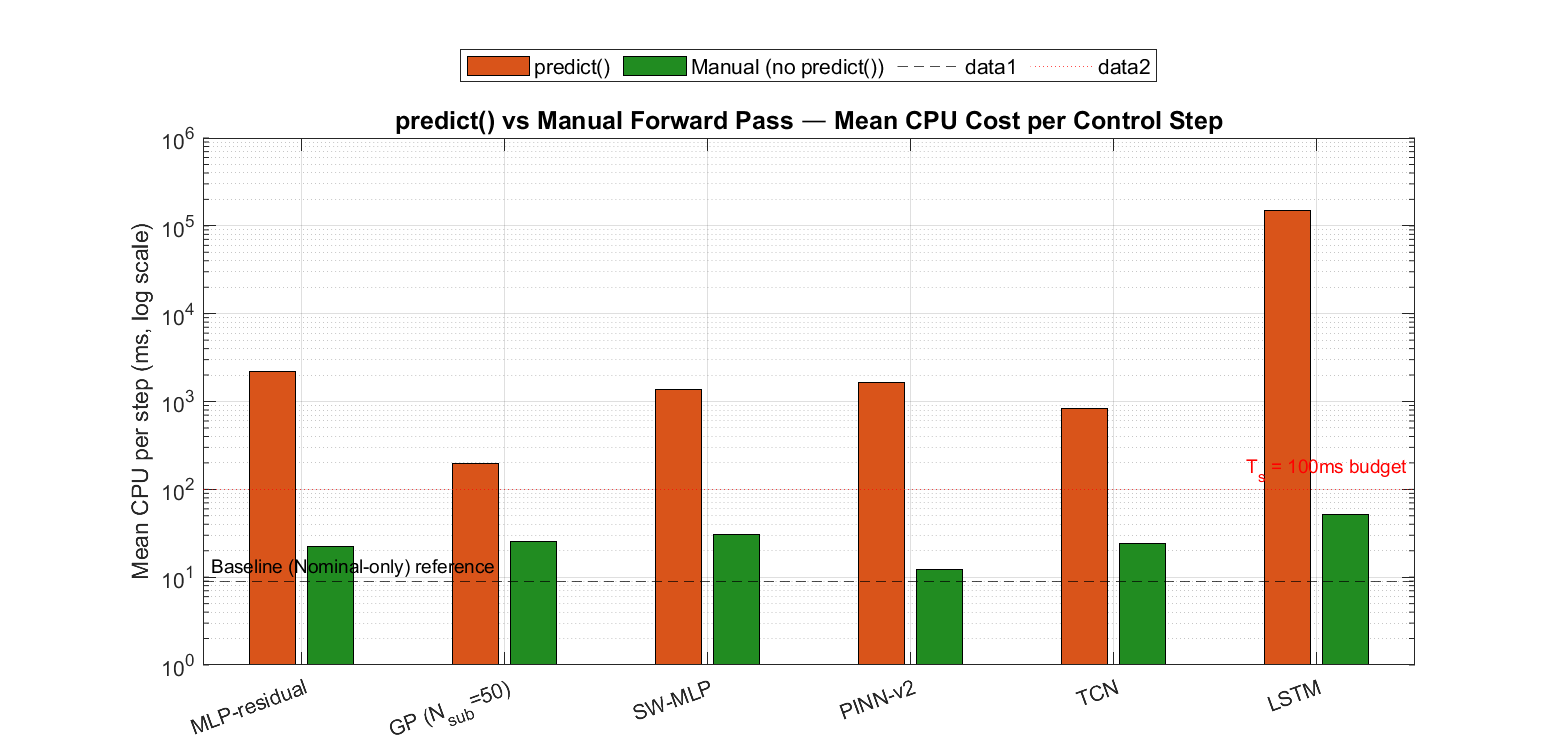
\includegraphics[width=0.85\textwidth]{figures/Fig1_PredictBypass_CPUComparison.png}
\caption{Mean per-step CPU cost, \texttt{predict()} versus manual
forward pass, all six surrogates (log scale), with the Baseline
reference and $T_s=\SI{100}{ms}$ real-time budget marked.}
\label{fig:predictbypass_cpu}
\end{figure}

\begin{figure}[H]
\centering
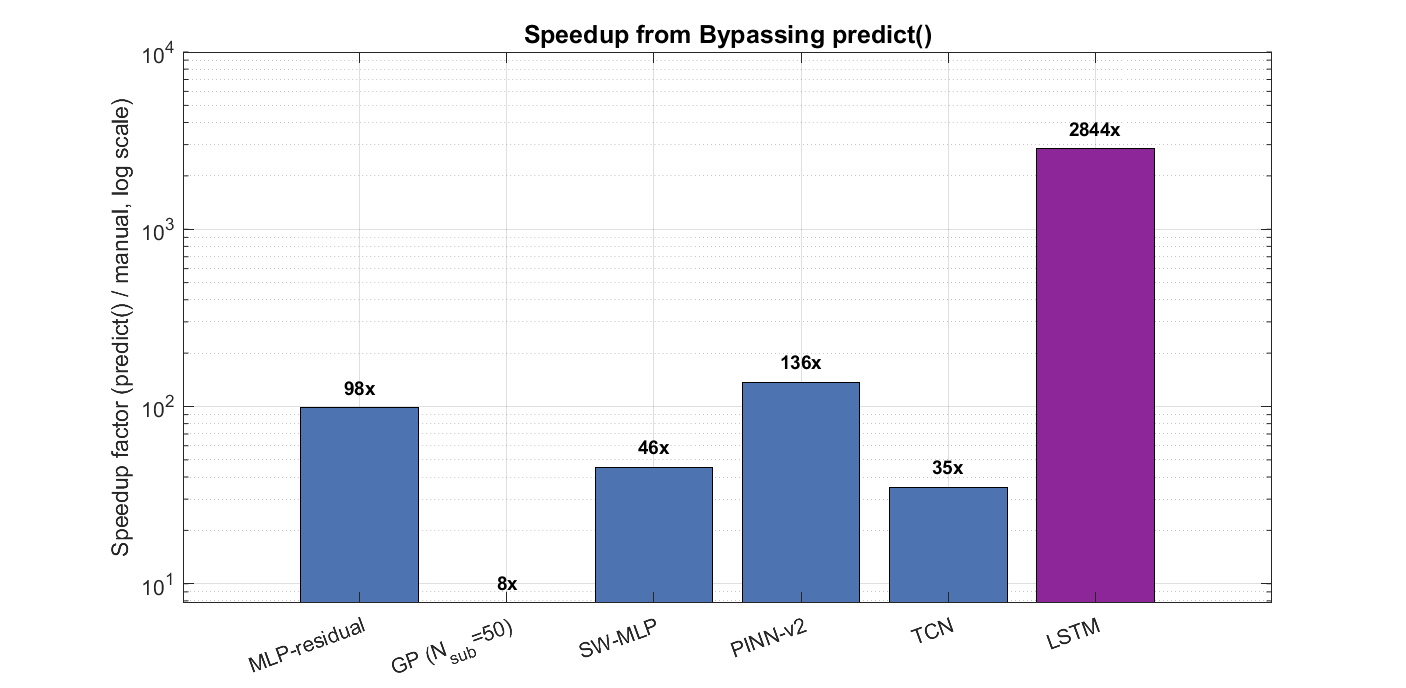
\includegraphics[width=0.8\textwidth]{figures/Fig2_PredictBypass_Speedup.png}
\caption{Speedup factor from bypassing \texttt{predict()}, all six
surrogates (log scale); LSTM (largest speedup, $2844\times$) highlighted.}
\label{fig:predictbypass_speedup}
\end{figure}

\begin{figure}[H]
\centering
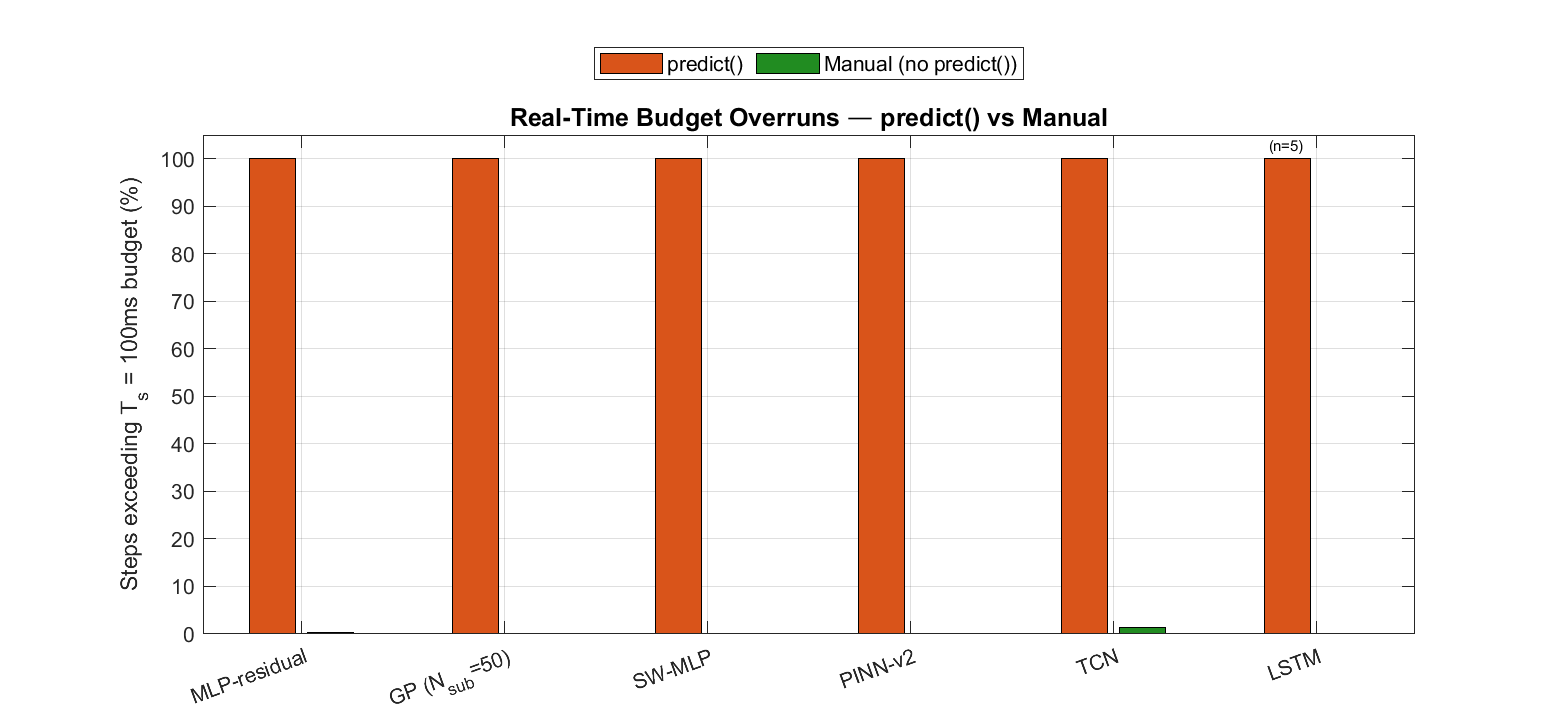
\includegraphics[width=0.85\textwidth]{figures/Fig3_PredictBypass_Overruns.png}
\caption{Real-time budget overrun rate ($T_s=\SI{100}{ms}$),
\texttt{predict()} versus manual forward pass, all six surrogates.}
\label{fig:predictbypass_overruns}
\end{figure}

Two results within Stage 4 are worth emphasizing. First, a
deliberately tiny residual-correction network (130 parameters, following
the nominal-plus-learned-correction structure of
\citet{aswani_provably_2013}) showed the \emph{same} catastrophic
\texttt{predict()}-based cost as the much larger TCN/GP/PINN-v2
surrogates (mean $\SI{2188.3}{ms}$/step), directly refuting network
size as the explanatory variable. Second, the initial manual
implementation of the TCN's causal convolution --- correct, verified to
$2.18\times10^{-7}$, but written as explicit triple-nested loops over
filters, timesteps, and kernel taps --- yielded only a modest $2.2\times$
speedup ($\SI{1319.2}{ms}\rightarrow\SI{437.6}{ms}$/step), with
overruns unchanged. Precomputing a reshaped weight matrix once at
extraction time and reformulating the convolution as a single matrix
multiplication per block (an ``unfold-and-multiply'' operation
standard in efficient convolution implementations) reduced this further
to $\SI{23.9}{ms}$/step ($56\times$ over \texttt{predict()}), matching
the Baseline's cost. This confirms that \emph{both} removing
\texttt{predict()}'s call overhead \emph{and} avoiding an unvectorized
manual re-implementation are independently necessary; verifying
numerical correctness alone is not sufficient evidence that a manual
bypass will be fast.

\paragraph{Stage 5 --- LSTM: the largest speedup, and the one
architecture that does not fully vanish.} LSTM shows both the most
extreme \texttt{predict()} cost ($\approx\SI{318}{s}$/step, consistent
with its highest isolated latency in Table~\ref{tab:isolated_benchmark})
and the largest bypass speedup ($2844\times$). Two aspects distinguish
this case from the other five. First, verifying the manual
gate-equation implementation (input/forget/cell-candidate/output gates,
MATLAB's standard ordering, applied recurrently over the
$L=10$-step window) against \texttt{predict()} yielded a consistently
small but non-negligible discrepancy ($1.3\times10^{-5}$--$2.0\times10^{-4}$
across five random test points), an order of magnitude larger than the
$10^{-7}$--$10^{-13}$ agreement found for the feedforward architectures
and GP. We attribute this to accumulated single-precision
(\texttt{dlnetwork}'s default, \texttt{float32}) versus
double-precision rounding compounding over ten sequential recurrent
steps of gate nonlinearities, rather than a logical error, since the
discrepancy is small and consistent in magnitude across independent
test points rather than an order-of-magnitude mismatch indicative of an
incorrect gate ordering.
\label{subsec:lstm_precision_note}
Second, and more fundamentally: unlike TCN's fixed-dilation
convolution, an LSTM's hidden and cell state at step $t$ depend
recursively on step $t-1$, so the ten-step window cannot be reduced to
a single matrix multiplication the way the convolution could. The
manual LSTM ($\SI{52.2}{ms}$/step) is consequently $\approx 2$--$4\times$
slower than the five single-pass architectures ($\SI{12}{-}\SI{30}{ms}$/step)
even after the \texttt{predict()} bypass, reflecting this irreducible
sequential cost rather than any remaining implementation inefficiency.

\paragraph{Synthesis.} Across all six surrogates, bypassing
\texttt{predict()} with a verified manual forward pass eliminates the
real-time budget violation that had appeared, in Stage 2, to be an
architectural incompatibility between deep-learning/GP surrogates and
SQP-based \texttt{nlmpc}. This finding is consistent with, and extends,
\citet{salzmann_real-time_2022}'s independent report that decoupling a
neural network's own evaluation from the surrounding MPC solver's
iteration loop is necessary to embed large learned models in real-time
optimal control --- our diagnostic identifies \emph{why} this
decoupling is necessary in this specific MATLAB toolchain
(\texttt{predict()}'s per-call overhead, not gradient cost or
model size) and \emph{quantifies} the remedy across six architecturally
distinct surrogates. Full closed-loop tracking results using these
manual-bypass controllers are reported in
Section~\ref{sec:closed_loop_results}.

